\documentclass[twoside,a4paper,12pt]{memoir}
\usepackage{a4}
\usepackage{times}
\usepackage{pslatex}
\usepackage{url}
\usepackage{mscthesis}
\usepackage{lipsum} % standard filler text, only needed for demo

\usepackage{listings}

\usepackage{rotating}
\usepackage{amsmath}
\usepackage[table,xcdraw]{xcolor}
\usepackage{tablefootnote}
\usepackage{tabulary}

% %% The package 'algorithm' is useful, but incompatible with memoir.
% %% Cor-Paul Bezemer / http://homes.esat.kuleuven.be/~dvherten/esatthesis.html
% %% suggest the following fix:
\let\newfloat\undefined \usepackage{algorithmic} 
\usepackage{algorithm}

% Include right (LaTeX/PDFLaTeX) graphics package
% (doesn't work under cygwin apperently)
%\ifx\pdftexversion\undefined
% \usepackage[dvips]{graphicx}
% \usepackage[dvips]{color}
%\else
\usepackage{graphicx}
% \usepackage[pdftex]{color}
%\fi

\usepackage{hyperref}

% Used in the bibliography to enable \citeauthor{citation}
\usepackage[numbers]{natbib}

% added by Mali
\usepackage{todonotes}

% Ensure that urls longer than the page width are broken up
% Based on the answer of StackOverflow user "xamde":
% https://tex.stackexchange.com/a/10401/155506
\expandafter\def\expandafter\UrlBreaks\expandafter{\UrlBreaks%  save the current one
  \do\a\do\b\do\c\do\d\do\e\do\f\do\g\do\h\do\i\do\j%
  \do\k\do\l\do\m\do\n\do\o\do\p\do\q\do\r\do\s\do\t%
  \do\u\do\v\do\w\do\x\do\y\do\z\do\A\do\B\do\C\do\D%
  \do\E\do\F\do\G\do\H\do\I\do\J\do\K\do\L\do\M\do\N%
  \do\O\do\P\do\Q\do\R\do\S\do\T\do\U\do\V\do\W\do\X%
  \do\Y\do\Z}

%---------------------------------------------------------------------%
%                     Options                                         %    
%---------------------------------------------------------------------%

\title{An Empirical Assessment on the Limits of Binary Code Summarisation with Transformer-based Models}
\subtitle{Version of \today}
% The final version of your thesis should typically use a different
% subtitle without the current date, for example
%\subtitle{Master's Thesis} 
% or remove the subtitle by uncommenting the following line: 
%\subtitle{}

\author{Ali Al-Kaswan}                               % CHANGE TO YOUR NAME
\authoremail{\url{a.al-kaswan@gmail.com}}       % CHANGE TO YOUR EMAIL ADDRESS
\birthplace{Lelystad, the Netherlands}                % CHANGE TO YOUR BIRTH PLACE
\studentid{4679678}                              % CHANGE TO YOUR STUDENT ID

% Optional for work done at a company, put this in comments if you did
% not do your thesis work at a company
\company{

\includegraphics[height=1.25cm]{img/ucd.png}\\
DECAL Lab\\
Faculty of Computer Science\\
University of California Davis\\
Davis, the United States\\
\url{www.cs.ucdavis.edu}
}

% Optional (postscript) cover picture. Put this in comments when not needed.
% \coverpicture{
\includegraphics[width=13cm]{img/maze.ps}}


% A copyright notice and maybe something about the cover picture
% Put in comments to get the default copyright notice
% \colophon{\noindent
%   \copyright{} \the\year \: \theauthor. \emph{Note that this notice is for demonstration
%   purposes and that the \LaTeX{} style and document source are free to
%   use as basis for your MSc thesis.} \\[1em] 
%   Cover picture: A ``random'' maze generated in postscript.
% }

% thesis committee:
\chair{Prof. Dr. A. van Deursen, Faculty EEMCS, TU Delft}
\supervisor{Dr. S. Verwer, Faculty EEMCS, TU Delft}
% The following two are optional for LaTeX (current university
% regulations state that at least one of them should be assigned)
\externalsupervisor{Prof. Dr. P. Devanbu, Faculty Computer Science, UC Davis}
\committeemembera{Dr. M. Izadi. Member, Faculty EEMCS, TU Delft}
\committeememberb{Dr. A. A. Sawant, Faculty Computer Science, UC Davis}


\setcounter{tocdepth}{1}
\setsecnumdepth{subsection}
\maxsecnumdepth{subsection}

\begin{document}
\frontmatter
\thispagestyle{empty}
% \maketitle                                      % for the cover page
\makeformaltitlepages{Reverse engineering binaries is required to understand and analyse programs of which the source code is unavailable. Decompilers can transform the largely unreadable binaries into a readable source code-like representation. Yet, during compilation and decompilation many aspects of source code, such as variable names and comments, are lost. Furthermore, by stripping the binaries, all other symbols, like the function name, are removed from the binary.

Reverse engineering is a time-consuming process, much of which is taken up by labeling the functions with semantic information \cite{reverseEngineerProcess}. We therefore propose a novel code summarization method applied to decompiled and stripped decompiled code. We leverage the existing BinSwarm dataset \cite{InlinedFunc}, which is further extended with aligned source code summaries. We create an artificial demi-stripped dataset, by removing the identifiers from unstripped decompiled code. We also fine-tune a pre-trained CodeT5 model for the code summarization task on the given dataset. Furthermore, we investigate the performance of the input types, the impact of data duplication and the importance of each aspect present in source code on the model performance. Finally, we design and present some intermediate-training objectives to increase the model performance.

We present the following findings: Firstly, we find that the model produces good summaries for decompiled code, with similar performance to source C code. The quality of the demi-stripped model was significantly lower but still usable. Stripped performed worse, and produced mostly incorrect and unusable summaries. Secondly, we find that deduplication greatly reduces the performance of the model, putting the performance of decompiled code roughly in line with other decompiled datasets \cite{CodeT5}. Third, we found that the loss of identifiers causes a drop in BLEU-4 score of 11.57 points, with another 8.16 decrease attributable to the increase of decompilation faults caused by stripping. Lastly, we present a Deobfuscation intermediate-training objective, which improved the performance of the model by 0.54 and 1.54  BLEU-4 on stripped and demi-stripped code respectively. }         % for formal title pages with all info

\chapter{\label{cha:Preface}Preface}

This is where you thank people for helping you etc.

 % add some pseudo content

\vskip1cm
\begin{flushright}
\theauthor\\
Delft, the Netherlands \\
\today\\
\end{flushright}



\cleardoublepage\tableofcontents
\cleardoublepage\listoffigures
\cleardoublepage\mainmatter

\chapter{Introduction}
\label{introduction}

% \begin{description}
% \item[Problem definition and Significance]: Reverse engineering binary programs can help to find vulnerabilities in software, this is a hard task that depends on the skill of the reverse engineer. Decompilers exist to help in this process, but their output is still difficult to read and understand. Making reverse engineering easier can help to find vulnerabilities, help researchers quickly understand novel malware, replicate software of which the source code is lost, discover illegitimate usages of intellectual property, porting abandonware, etc. Current approaches mainly focus on the recovery of aspects which are lost in the compilation and decompilation process such as names and types. This fails to address the need for methods to increase the comprehensibility of decompiled code.


% \item[Main Contributions] We, therefore, propose our code summarization solution, which takes decompiled functions and synthesises summaries. Our main contributions are a pre-trained fine-tuned code-summarization model. To create this model we explored the influence of the input types, the impact of data duplication, the impact of different aspects of stripped code and intermediate training on the model performance. We also provide a novel dataset with aligned source code, decompiled code and comments, for both stripped and unstripped code.
% \end{description}
% \newpage

\section{Problem Definition and Significance}
Reverse Engineering (RE) the inner workings of binary executables is required to analyse and understand programs. Furthermore, it can be used to find vulnerabilities and to analyse novel malware. Besides from analysing malware and finding vulnerabilities, reverse engineering can be used to find vulnerabilities, help researchers quickly understand novel malware, it can help with fingerprinting existing malware \cite{TypeInferenceSurvey}, replicate software of which the source code is lost, discover illegitimate usages of intellectual property, porting abandonware, and more\cite{TypeInferenceSurvey}. Furthermore, the binaries are the most accurate representation of the program that actually runs on the system, there is no guarantee that the source code actually represents the binary that is delivered to the user \cite{TypeInferenceSurvey}.

Unlike binaries, the source code is relatively easy to read. The source code of the binaries is, however, not always available. The original source code gets compiled into a runnable binary program by compilers such as Clang/LLVM \footnote{Clang: https://clang.llvm.org/} or GCC \footnote{GCC: https://gcc.gnu.org/} and delivered to the user.

To understand what a binary program does exactly, the binary code can be decompiled into readable code by decompilers such as Ghidra\footnote{Ghidra Framework: url{https://ghidra-sre.org/}} and IDA Pro\footnote{IDA Pro: url{https://hex-rays.com/ida-pro/}}. Understanding decompiled code is still an intrinsically difficult process. It is a manual, time-consuming process and still largely depends on the skill of the Reverse Engineer\cite{TypeInferenceSurvey}.

A large part of the work that goes into reverse engineering a binary is spent labelling functions with semantic information \cite{reverseEngineerProcess}. In the source code domain, automatic code-summarization  \cite{recommend_summarization} is used to automatically generate short natural language descriptions of source code. The summaries generated by these models are supposed to mimic the single-sentence comments or descriptions that are included in the source code. While these methods have been successfully applied syntactically rich to programming languages such as Python, Java and PHP\cite{CodeT5, CodeBERT, CodeX}, none of these methods has been applied to the relatively syntactically-poor output of decompilers. Especially stripped binaries, binaries of which the symbol table is removed, will prove to be challenging since they have almost no identifiers at all.

\subsection{Stakeholders}
There are several stakeholders who might benefit from this research. 
\begin{enumerate}
    \item Firstly, security researchers who aim to understand malware. This could help them understand and reverse engineer novel malware more quickly.
    \item Users of closed-source software can use this to inspect the software for faults. Closed source software can be patched, rewritten and reused to serve their exact purposes. Furthermore, an understanding of the source code can allow users to change the binary in memory during runtime. A malicious example of this group is game hackers who change certain memory addresses to give themselves an unfair advantage (changing their health points for instance) \cite{TypeInferenceSurvey}. 
    \item Reverse engineers who aim to replicate closed-source software or software of which the source code is lost. Reverse engineering can be used to help create open-source copies or to port the software to newer architectures. Examples range from porting old abandoned open-source projects to porting abandonware (on which copyrights still apply), or even the theft of intellectual property from closed-source commercial software.
    \item On the flip side, creators of closed-source software can use reverse engineering to determine whether other software has copied their products and infringed on their intellectual property.
    \item Lastly, developers of reverse engineering programs and toolkits might be able to use the results of this research to enhance their own products. 
\end{enumerate}

\section{Goal}
Below follows the goal for this master thesis:\\

\centerline{\textbf{To assess the application of the code summarization task on decompiled code.}}

\section{Contributions}
We therefore propose our code summarization model, which takes decompiled functions and synthesises summaries \ref{fig:useCase}. The starting point for a reverse engineer is a binary that has been compiled by a compiler from source code. This binary is then processed by a reverse engineering tool like Ghidra, which decompiles the binary. From this decompiled code the functions are then extracted. These decompiled functions are then summarised using our trained CodeT5 \cite{CodeT5} model.

\label{fig:useCase}
\begin{figure}[htb]
    \centering
    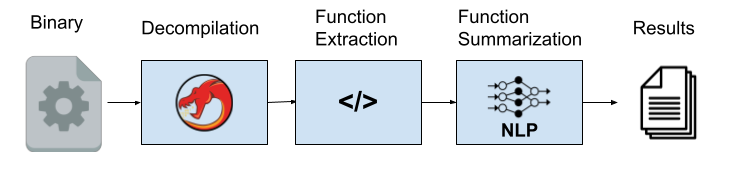
\includegraphics[width=\textwidth,height=\textheight,keepaspectratio]{img/UseCase.png}
    \caption{Proposed solution}
\end{figure}

We perform experiments on this solution to find the impact of decompilation and stripping on the model performance. Furthermore, we investigate the impact of duplicates in the data, as well as investigate which differences between stripped and unstripped data contribute most to the performance drop. Finally, we use the knowledge gathered by these experiments and design intermediate-training objectives to improve the preformance of the model on stripped decompiled code.\\

\textbf{Our main contributions can be summarised as follows:}
\begin{description}
 \item[Model:] Our main contribution is a pre-trained fine-tuned code-summarization model for decompiled and stripped-decompiled code. The model uses CodeT5 and is fine-tuned and evaluated on our own dataset of source code, decompiled code and stripped-decompiled code pairs. 
 \item[Impact study:] To create this model we explored the influence of the input types, the impact of data duplication, and the impact of different aspects of stripped and unstripped decompiled code on the model performance.
 \item[Intermediate-training:] To improve the performance of the model we implemented and evaluated the Neural Machine Translation (NMT), deobfuscation (DOBF) and span-detection (SPAN) intermediate-training objectives. 
 \item[Dataset:] Finally, we contribute the dataset used to fine-tune and pre-train the model. The dataset contains aligned comment-source code, comment-decompiled code, and comment-stripped-decompiled code pairs. We also provide a synthetic dataset of comment-demi-stripped code pairs. Furthermore, we provide the data used by the pre-training objectives. This is a novel dataset which can be used by other works to train and evaluate their models.
\end{description}

\section{Structure}
The rest of the thesis is outlined as follows: Chapter \ref{background} will consist of a brief introduction and explanation of concepts and tools used throughout the thesis. In chapter \ref{relatedWork} we will discuss other relevant works in this field. Chapter \ref{methodology}  will cover the research methodology, the experimental setup will be covered in chapter \ref{ExperimentalSetup}. The results will be presented in chapter \ref{results}, followed by a discussion on the findings and feature a short discussion on the threats to validity in chapter \ref{discussion}. Finally, chapter \ref{conclusion} will conclude on the findings and discuss possible future works.

\chapter{Background}
\label{background}
Explain relevant concepts needed to understand the experiments and findings:\\

Binary Reverse Engineering:
\begin{itemize}
    \item Compilers and compiler levels
    \item Stripping
    \item Ghidra
\end{itemize}

NLP for code:
\begin{itemize}
\item Code Summarization
\item Transformers and CodeT5
\item Scoring methods
\end{itemize}

\newpage
\section{Binary Reverse Engineering}

\subsection{Compilers and Optimization Levels}
Compilers are programs that translate code from one language to another, but generally and in the context of this thesis, the term is used to refer to programs that translate high level code like C to a lower level language such as machine code. For our work we focus on the GNU Compiler Collection (gcc)\footnote{gcc: \url{https://gcc.gnu.org/}} and Clang/LLVM (Clang)\footnote{Clang: \url{https://clang.llvm.org/}}.

Compilers frequently feature optimization levels. Generally the goal of optimizations is the improvement of runtime performance or program size at the expense of compilation time and ability to debug \cite{ColeOptimizationLevel}. Compilers generally use optimizations, grouped into optimization levels, where each level uses a different set of optimizations.

For example, the gcc features 60 optimizations across 8 different optimization levels, which are denoted by a -O option \cite{ColeOptimizationLevel, gccOptimization}. By default, if gcc is invoked without any optimization options, the program will be compiled with O0. O1, 02 and O3 incrementally apply more optimization to the binary at the expense of a higher compilation time \cite{gccOptimization}. These optimization levels are also found in other compilers such as Clang-LLVM. Other optimization levels, such as Os, which optimizes for binary size, are also included in gcc \cite{gccOptimization}.

Optimizations can restructure and transform the program in relation to the source code, by changing the control flow or the data of the program \cite{optimizationObfuscation}. This obfuscation can complicate the reverse engineering process by reducing the accuracy of Ghidra \cite{optimizationObfuscation}.  

\subsection{Ghidra}
Ghidra is a free and open source reverse engineering toolkit developed by the US National Security Agency. Ghidra has been in development since the turn of the century and had been in use internally. Its existence was leaked by Wikileaks in March of 2017 and the tool was released to the public in March of 2019, before being open sourced in April of the same year.

Ghidra contains many separate analysis modules that allow a reverse engineer to analyse compiled code. The modularity of Ghidra and the inclusion of a scripting engine allow users to add custom modules and scripts. We will specifically focus on the tools used in the process that was used to transform binaries into readable code (see \ref{fig:ghidra}).

\label{fig:ghidra}
\begin{figure}[!h]
  \centering
  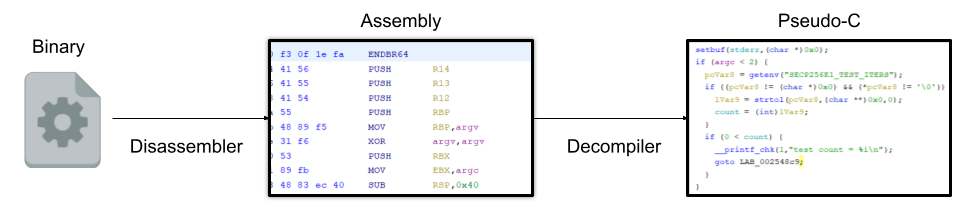
\includegraphics[width=\linewidth]{img/ghidra.png}
  \caption{Transformation of binary to readable code.}
\end{figure}

Ghidra features a disassembler \ref{fig:disassembler}, which will take the binaries and assemble them back into an intermediate representation. In the case of x86-x64 binaries like the binaries this project will focus on, this intermediate representation will be assembly. Processors have an associated language that defines the mapping
between user readable assembly language instructions (e.g. MOV, ADD, etc.) and their corresponding byte values. In order to properly disassemble a binary image for a specific architecture, Ghidra requires a language module for that specific processor. A language module is the software that implements the language translation. Ghidra has a set of language modules for the most popular processor languages(such as x86-64, ARM. MIPS ..). Besides these out-of-the-box supported architectures, developers have also been extending Ghidra's support with custom processor architectures. 
\label{fig:disassembler}
\begin{figure}[!h]
  \centering
  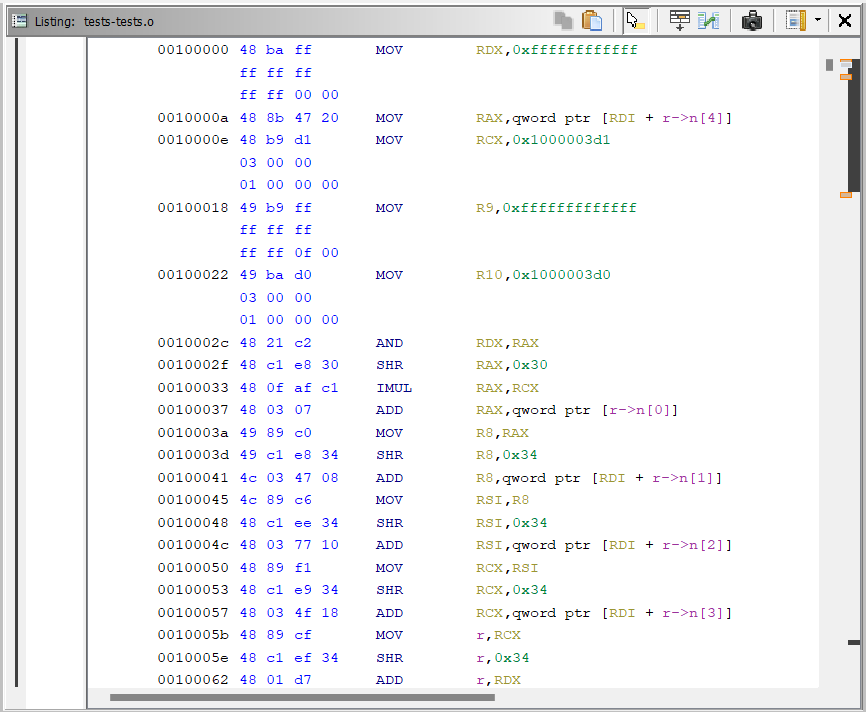
\includegraphics[width=\linewidth]{img/disassembler.png}
  \caption{Ghidra's disassembly window.}
\end{figure}

The decompiler, also featured in Ghidra \ref{fig:decompiler}, is a processor language-agnostic transformation engine that takes the disassembled code and creates a source code representation. The representation is in pseudo-C, a C-like representation that generally follows the general language conventions of C. The interactive decompiler window allows the user to directly see the correspondence between the pseudo-C and assembly representation. The user can also make changes to the decompiled code, such as changing automatically generated variable names and types and adding comments. 

\label{fig:decompiler}
\begin{figure}[!h]
  \centering
  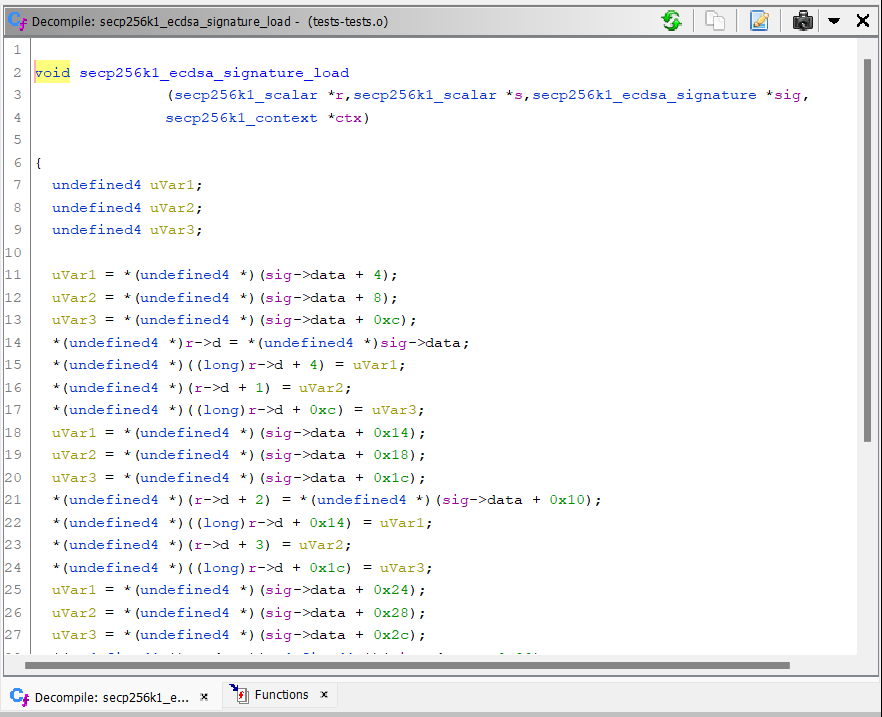
\includegraphics[width=\linewidth]{img/decompiler.png}
  \caption{Ghidra's decompiler window showing a snippet of decompiled function from the secp256k1 ECDSA library}
\end{figure}
\newpage
\subsection{Stripping}
Aside from compiling with higher optimization levels, binaries can also be stripped to obfuscate the underlying code and to resist analysis\cite{StochFuzz}. Binaries which have not been stripped still contain a lot of debug information, which can be used during development. This debug information, like function names, self defined types etc., can be used to analyse and reverse engineer the binary. Commercial Off-the-Shelf (COTS) software is often stripped to reduce the memory and storage footprint of binary, and to resist analysis to protect the intellectual property of the creator. Many vulnerable and malicious binaries are, unfortunately, also stripped to resist security analysis and hide their faults\cite{Debin}.

Unix and Unix-like operating systems include a strip utility. The strip utility removes any operands that are not necessary for the execution for the binary, while ensuring that the execution of the binary remains unchanged, the exact implementation and scope of the utility is left to the implementation\footnote{strip: \url{https://pubs.opengroup.org/onlinepubs/007908799/xcu/strip.html}}. 

The strip utility as implemented in GNU/Linux, removes the symbol table from the binary. The symbol table contains the symbol location, type and name. The symbol table can be dumped for a given binary by using the nm command \ref{fig:nm}, which is included in Unix and Unix-like operating systems \footnote{nm: \url{https://pubs.opengroup.org/onlinepubs/9699919799/utilities/nm.html}}. 

\label{fig:nm}
\begin{figure}[!h]
  \centering
\begin{lstlisting}
                 U malloc
                 U memcpy
                 U memset
0000000000000060 r minus_b1.3052
0000000000000040 r minus_b2.3053
0000000000005680 t nonce_function_rfc6979
00000000000000c1 r one.4283
0000000000000120 r output32.4535
00000000000000e0 r pad.4239
00000000001101e0 r secp256k1_const_lambda
0000000000110240 r secp256k1_const_modinfo_fe
0000000000110200 r secp256k1_const_modinfo_scalar
000000000000c7d0 T secp256k1_context_clone
000000000000c690 T secp256k1_context_create
000000000000c920 T secp256k1_context_destroy
0000000000000000 D secp256k1_context_no_precomp
...
\end{lstlisting}
  \caption{Sample output of nm command from secp256k1 \protect\footnote{Bitcoin secp256k1: \protect\url{https://github.com/bitcoin-core/secp256k1}} ECDSA library}
\end{figure}
% FIX THIS, footnote doesnt work

Like higher optimization levels, the use of stripping can greatly complicate the efforts to reverse engineer a binary, as well as reduce the accuracy and effectiveness of reverse engineering tools. 
\section{NLP for Code}

\subsection{Code Summarization}

\subsection{Transformer and CodeT5}
The current state-of-the-art natural language programming language processing models such as CodeT5 \cite{CodeT5}, CodeBERT \cite{CodeBERT} and CodeX \cite{CodeX} are all based on the Transformer architecture \cite{Transformers}.

Pre-trained language models, such as RoBERTa, CodeBERT \cite{CodeBERT} and CodeT5 \cite{CodeT5} utilize a pre-train and fine-tune paradigm. In this paradigm the models are first trained in an unsupervised manner on a large unlabeled dataset. In the case of RoBERTa, a Masked Language Modeling (MLM) objective was used, where random tokens are masked out from a swath of text (or CodeBERTs case code) and the model is tasked to predict said tokens.

\subsection{Scoring Methods}
\chapter{Related Work}
\label{relatedWork}
Discuss the different works in the field of binary reverse engineering:

\begin{description}
    \item[Debin] \textcite{Debin} use a statistical model to predict variable names from stripped assembly. But suffers from poor generalizability and poor performance on other datasets \cite{VarBERT}[p.1]
    \item[Dire] \textcite{Dire} use an LSTM and A GNN to predict variable names and types from stripped binaries.
    \item[VarBERT] \textcite{VarBERT} uses a BERT model, pre-trained with a constrained MLM objective, to predict variable names and types
    \item[Neutron] \textcite{Neutron} apply Machnine Translation to translate from decompiled (not stripped) code back to source code using an LSTM  
    \item[FUNCRE] \textcite{InlinedFunc} apply pre-training and fine tuning to a RoBERTa model to identify and recover usages of inlined functions in decompiled code
    \item[SnowWhite] Recently, \textcite{SnowWhite} used a statistical model to predict types from webassembly binaries
    \item[StochFuzz] Recently, \textcite{StochFuzz} applies the use of fuzzers, to analyse stripped binaries for vulnerabilities, but the fuzzer only finds vulnerable inputs and does not give any insight into the binary itself
\end{description}

From these works none focus on the summarization of stripped binaries, they either focus on the recovery of certain aspects lost by stripping or on the translation of unstripped code back to source code.
\chapter{Methodology}
\label{methodology}
\todo[inline]{This can be renamed to approach}

% \begin{itemize}
%     \item Explain the data collection step, and how the comments were collected and aligned using BinSwarm. 
%     \item Explain the deduplication methods used and why duplicates in this task are fine, but why we choose to report the deduplicated results anyway.
%     \item Explain the experimental setup for the standard model, how we pre-processed the data, fed it into the model and the evaluation 
%     \item Explain the experimental setup for the pre-training, the translation, DOBF and span detection, how and why the pre-training steps were done, and how they were evaluated
% \end{itemize}
% \newpage
In this chapter the methodology of our solution is discussed in detail. More specifically, we start with a discussion on data collection step, how the data was aligned and prepared. Followed by a discussion on the intermediate-training set-up. Finally the fine tuning of the model will be covered.

\todo[inline]{first provide an overview of the proposed approach in 1-2 paragraphs, then layout the structure of chapter and finally go into more details}

\todo[inline]{you can include a running example to walk the reader through your approach, it makes it much easier to understand the work}

\section{Data Collection}
To create and assess our solution we require a dataset of decompiled functions labeled with a description. This dataset should be relatively large to suit the "data-hungry" deep-learning models that we utilize. Furthermore the dataset needs to feature a diverse set of data, representative of the actual real-life usecase of our solution. 
To create a large and diverse dataset to train and assess our solution we made use of BinSwarm \cite{InlinedFunc}, an existing dataset of aligned decompiled and stripped decompiled functions \footnote{BinSwarm; \url{https://hub.docker.com/r/binswarm/cbuilds}}.

Buildswarm starts by collecting C-based projects from Github. The projects are filtered to only include projects that are: Actively being developed, using Travis CI and built for Ubuntu Linux. The projects are then built using Docker. The resulting binaries are then stripped and both the stripped and unstripped binaries are decompiled using Ghidra, the functions are extracted from the decompiled code and aligned with the source code. 

To add descriptive comments to this dataset, we extract documentation from the original source code. We depend on the documentation that was included in the source code by the original authors in the form of single and multiline comments. The decompiled functions are alligned with the comments in the source code by using srcML to extract any documentation located directly before a function signature, and then finding the function signature and project name in the decompiled dataset.

The documentation of a function often also contains other details aside from the descriptive summary. We found that C projects do not follow a single documentation standard. Javadoc for Java has a short one line description or summary for each method at the beginning of the multiline comment. In C there is no singular documentation standard so there might not be a single line summary and we will need t automatically locate it in the comment block. 
Furthermore, we found that a large number of function did not have any documentation associated with them. To deal with these issues we did not include any functions that are missing any documentation. To find the single line description we devised a few simple rules to extract the summary.

A high level overview of this process can be found in figure \ref{fig:dataCollection}.

\label{fig:dataCollection}
\begin{figure}[!h]
  \centering
  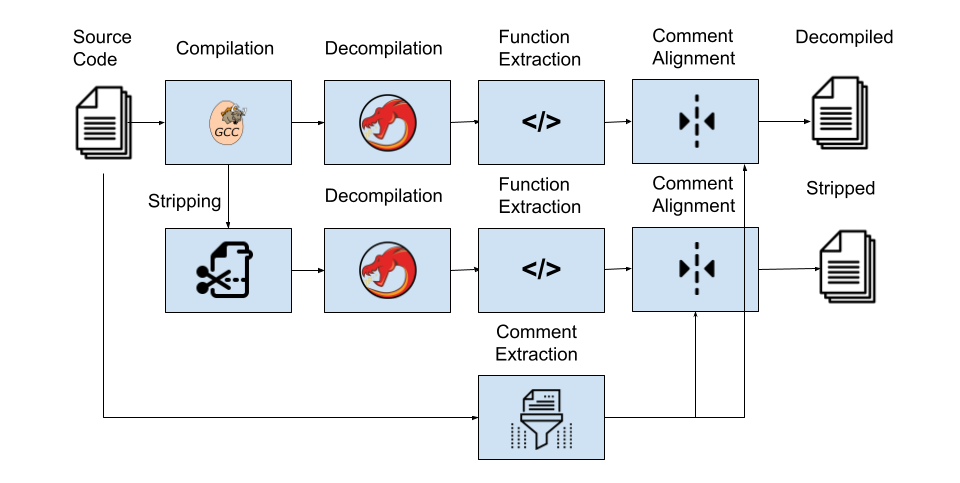
\includegraphics[width=\linewidth]{img/dataCollection.png}
  \caption{Data Collection}
\end{figure}

From the dataset of decompiled functions another dataset is also created. We can emulate the process of stripping by removing all the identifiers from the decompiled code and replacing them with placeholders, for the purpose of clarity, we call this demi-stripped data. Like the stripped dataset, the identifiers are all removed, but the decompiler still had access to the identifiers and could use the symbol table during decompilation. Most importantly, this demi-stripped dataset still has the same structure and control flow as the unstripped decompiled dataset.

\subsection{Dataset Split}
The dataset is split into a train, test and validation set. These sets constitute approximately, 80\%, 10\% and 10\% respectively\cite{recommend_summarization} of the complete dataset. To prevent leakage of vocabulary and code patterns between the sets, we sample the sets in a cross-project manner. Meaning that an entire project gets assigned to one of the sets, and functions from the same project cannot be assigned to different sets. The different sets should also have a similar distribution of optimization level and average source-code length.

\subsection{Duplication}
Large corpora of code, like the corpus gathered by BinSwarm, tend to have a high degree of duplication \cite{leclair_recommendations}. Snippets of code that are relatively unchanged appear in multiple parts of the corpus. This can be in the form of functions that are copied, generic or auto-generated. These functions will then appear in multiple repositories and might be duplicated across the training and testing data.

Besides exact duplicates, near-duplicates can also occur. Near-duplicates are like exact duplicates but they differ in a few small aspects like different code comments or different function names. While removing exact duplicates is relatively fast and straightforward, removing near-duplicates is a much harder and computationally intensive \cite{allamanis_adverse}. 

The issue with code duplication in classical code summarization is that the models and tools are supposed to be used to generate summaries for new and unseen code. The evaluation metrics should therefore measure the generalization of the tool on new samples \cite{allamanis_adverse}. Duplicates and near-duplicates are not defined as new samples, a user of such a tool could simply look these samples up. Furthermore, large, high-capacity models like CodeT5 with 220 million or Codex 12 billion \cite{CodeX} trainable weights \cite{CodeT5}, have a large capacity to memorize duplicated code \cite{allamanis_adverse}.
The usecase outlined in this work, is however, more akin to deobfuscation. As explained by Allamanis, deobfuscation could be a usecase where duplicates are valid and part of the true distribution of the problem\cite{allamanis_adverse}. Compiled code contains a lot of duplicate code, and understanding this code is still difficult and of importance towards the understanding of the binary. We will therefore focus on the performance of the model on code with duplicates, but we will also report the deduplicated results.

\section{Intermediate-Training}
The standard CodeT5 model was not pre-trained on any decompiled code, it might therefore be useful to apply additional training steps to 'teach' the model the embedding of decompiled and stripped decompiled code. Since we apply these training steps between the pre-training and fine-tuning of the model, we refer to this training strategy as intermediate-training.

To apply and assess other intermediate-training objectives we train a CodeT5-base model on a predefined objective, then after that intermediate-training step, we fine-tune the resulting model on our fine-tuning datasets. We essentially apply another training step to the already pre-trained base model. We can then measure the impact of the intermediate-training step on the performance of the model after fine-tuning.

\label{fig:preTraining}
\begin{figure}[H]
  \centering
  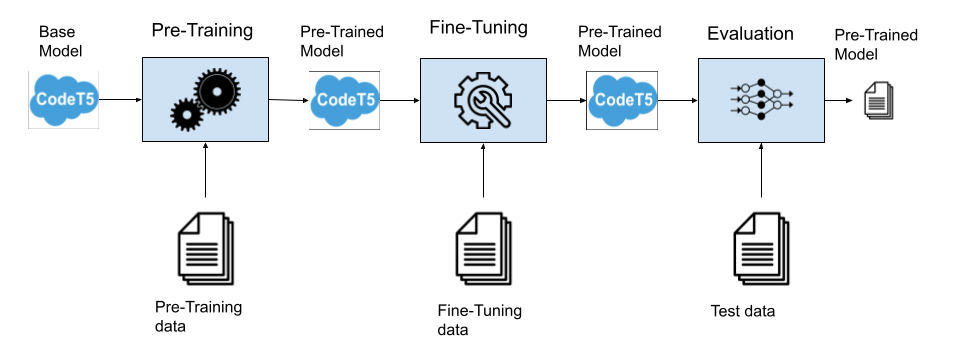
\includegraphics[width=\linewidth]{img/pre-training.png}
  \caption{Pre-Training}
\end{figure}

We define and a number of different pre-training objectives. Each of these objectives aims to teach the model the embedding of the identifiers, such that these identifiers can be inferred on the stripped code. For these objectives we make use of the relatively large dataset of demi-stripped code, to prevent leakage we remove the test set of the stripped code from the dataset.

\section{Fine-Tuning}
The concept of transfer learning, which is utilized in CodeT5 depends on the use of a fine-tuning step to train the pre-trained model on the downstream task. In this case we make use of the CodeT5-base model which was trained on the mixed upstream tasks by the authors \cite{CodeT5}.

We fine-tune a pre-trained CodeT5-base model on the constructed dataset. The model is trained on the summarization task as defined in the model. The model is trained on the train set, then evaluated after every epoch on the validation set and finally tested on the test set. The performance of the model is measured using the EM (exact match), BLEU-4 scores.
\chapter{Experimental Setup}
\label{ExperimentalSetup}
% \begin{itemize}
%     \item We aim to answer the following questions:
%     \begin{itemize}
%         \item RQ1: How do different input types (source, unstripped decompiled, demi-stripped, stripped) affect the model's performance (data-richness effect)?
%         \item RQ2: What is the impact of data duplication on the model's performance (data-duplication effect)?
%         \item RQ3: To what extent each aspect of stripped decompiled binaries impacts the model's performance (data-input study)?
%         \item RQ4: How do different pre-training objectives affect the model's performance (model-objective effect)?
%     \end{itemize}
%     \item Explain what script was used for deduplication
%     \item Explain how the model was loaded in and what configurations were used
%     \item Explain which metrics we used to assess the model
%     \item Explain the manual evaluation of the stripped code
%     \item Explain the baseline of CodeT5 on normal programming languages, and our own finetuning on source-C
% \end{itemize}

% \newpage

\section{Research Questions}
To create and assess our model and contributions, we define the following research questions which will be answered throughout the thesis.
\todo[inline]{you can first add a bit of story here to connect the RQs together, then go to the details of each question}

\begin{itemize}
    \item \textbf{RQ1: How do different input types (source, unstripped decompiled, demi-stripped, stripped) affect the model's performance? (data-richness effect)}
    \begin{sloppypar}
    Firstly, we want to know how the impact of the data-richness on the model performance. The different datasets that we have different degrees of data richness, the source-code has all of its identifiers and has comments in the code. Unstripped decompiled code has no comments and loses many of its identifiers, some noise is also introduced by the decompiler. Demi-stripped data loses all of the remaining identifiers. Stripped data, also has no identifiers and introduces even more decompilation noise.
    \end{sloppypar}
    \item \textbf{RQ2: What is the impact of data duplication on the model's performance? (data-duplication effect)}
    \begin{sloppypar}
    Secondly we will evaluate how the model reacts to data duplication, whether the model performance is simply a result of the memorization of certain examples, or if the performance is a result of a generalizable understanding of the data.
    \end{sloppypar}
    \item \textbf{RQ3: To what extent each aspect of stripped decompiled binaries impacts the model's performance? (data-input study)}
    \begin{sloppypar}
    The different datasets each contain different aspect of the original source code, which of these aspects are most important towards the model performance? 
    \end{sloppypar}
    \item \textbf{RQ4: How do different pre-training objectives affect the model's performance? (model-objective effect)}
    \begin{sloppypar}
    Finally, we will apply the insights provided by the previous questions to design new pre-training objectives, through which we aim to address the shortcomings of the base-model. 
    \end{sloppypar}
\end{itemize}

\section{Dataset}
To answer the research questions a diverse and representative dataset must be constructed. The Buildswarm dataset contains around 1.8m aligned decompiled-sourcecode pairs as well as 400k aligned stripped-sourcecode pairs. The large difference is caused by the inherent difficulty of finding functions in stripped decompiled code. 

From this dataset we collect any documentation that is located above the functions using srcML \ref{fig:srcML}. 
\label{fig:srcML}
\begin{figure}[H]
  \centering
  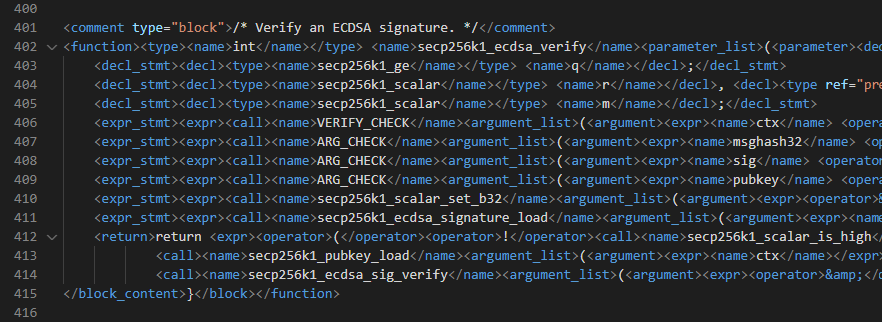
\includegraphics[width=\linewidth]{img/srcML.png}
  \caption{Example function with its documentation (truncated)}
\end{figure}

This documentation can be split into the following classes: 
\begin{enumerate}
  \item Double slash comments, example from Jep:release\_utf\_char. 
\begin{verbatim}
    // release memory allocated by jstring2char
\end{verbatim}
    These comments are thrown out, as these are generally not used for documentation.
  \item Single line comments, example from Nesbox:Curl\_mime\_read.
\begin{verbatim}
    /* Set mime part remote file name. */
\end{verbatim}
   We take the entire comment as a description.
  \item Multiline comments, example from oftc-ircservices:cs\_on\_client\_join.
\begin{verbatim}
    /**
     * CS Callback when a Client joins a Channel
     * @param args 
     * @return pass_callback(self, struct Client *, char *)
     * When a Client joins a Channel:
     *  - attach DBChannel * to struct Channel*
     */
\end{verbatim}
    In this case we take the first line or sentence.
\end{enumerate}



The data is pre-processed using the Pandas \footnote{Pandas: \url{https://pandas.pydata.org/}} data analysis library as well as the Pandarallel \footnote{Pandarallel: \url{https://pypi.org/project/pandarallel/}} parrallelizability extention for Pandas.

The samples are pre-processed by first extracting the function name and adding it as a column to the data, for the stripped samples the allignment with C is utilized by extracting the function name from the sourcecode for each of the samples. The samples are aligned with the comment data using the name of the file where they reside appended with the function name, for instance: \textit{/Repos\_Bionic/ secp256k1/secp256k1.c :secp256k1\_pubkey\_load}. We further pre-process the data by removing any newlines from the function body and by unescaping any characters that have been escaped for file safety purposes such as \&gt; for $>$.

The samples are split into a train, validation and test set. Each set is collected into a single .jsonl \footnote{JSON Lines: \url{https://jsonlines.org/}} file.

\label{fig:jsonl}
\begin{figure}[H]
  \centering
  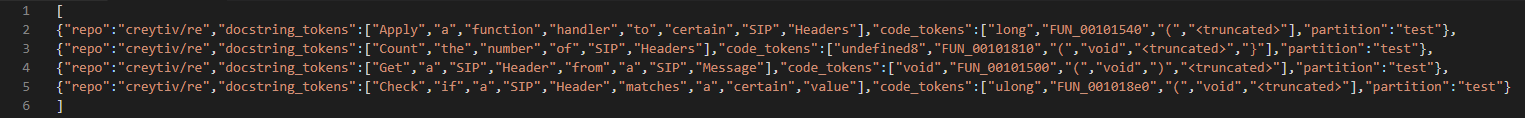
\includegraphics[width=\linewidth]{img/jsonl.png}
  \caption{Example entries of a .jsonl file used to train/evaluate code summarization from stripped code, for brevity the function body has been truncated.}
\end{figure}

\subsection{Deduplication}
\todo[inline]{you can avid the header here. also you can move all the libraries and tools that you used to the configuration/implementation details subsection (under experimental setting). note that you can explain the general process here, but it is better to move the details of implementation under one subsection (configuration/implementation). also make sure that you do not repeat content from data set collection in the "methodology" chapter.}


To answer the second research question the dataset must be deduplicated. The dataset is deduplicated using a fork\footnote{Near Duplicate Code Detector: \url{https://github.com/SERG-Delft/near-duplicate-code-remover}} of the near-duplicate-code-detector \cite{allamanis_adverse}. We use this tool to compare all the functions in the dataset and to find clusters of near-duplicate functions. We randomly select one function per cluster and discard the rest from the dataset. 

% Slightly expand this 

\section{Model Configuration}
To first establish a performance baseline we trained a CodeT5-base model on the summarization task on the source C. This can be used to compare the decompiled C, stripped decompiled C and the demi-stripped datasets to source code. For deduplicated code, the results can be compared with the performance of CodeT5-base on the code summarization task \ref{tab:codeT5Baseline}, where the performance varies between 15.24 and 26.03 BLEU4 score depending on the language \ref{tab:codeT5Baseline}. Based on this, and table \ref{tab:BLEUScale} we set the baseline for a usable summarization model around a BLEU4 score of 15, with anything lower than a BLEU4 score of 10, essentially unusable.


We also trained the model on the deduplicated datasets. 
\label{tab:codeT5Baseline}
\begin{table}[H]
\centering
\begin{tabular}{|l|llllll}
\hline
\rowcolor[HTML]{C0C0C0} 
Model                 & \multicolumn{1}{l|}{\cellcolor[HTML]{C0C0C0}Ruby} & \multicolumn{1}{l|}{\cellcolor[HTML]{C0C0C0}Javascript} & \multicolumn{1}{l|}{\cellcolor[HTML]{C0C0C0}Go} & \multicolumn{1}{l|}{\cellcolor[HTML]{C0C0C0}Python} & \multicolumn{1}{l|}{\cellcolor[HTML]{C0C0C0}Java} & \multicolumn{1}{l|}{\cellcolor[HTML]{C0C0C0}PHP} \\ \hline
Seq2Seq               & 9.64                                              & 10.21                                                   & 13.98                                           & 15.93                                               & 15.09                                             & 21.08                                            \\ \cline{1-1}
Transformer           & 11.18                                             & 11.59                                                   & 16.38                                           & 15.81                                               & 16.26                                             & 22.12                                            \\ \cline{1-1}
RoBERTa               & 11.17                                             & 11.90                                                   & 17.72                                           & 18.14                                               & 16.47                                             & 24.02                                            \\ \cline{1-1}
CodeBERT              & 12.16                                             & 14.90                                                   & 18.07                                           & 19.06                                               & 17.65                                             & 25.16                                            \\ \cline{1-1}
PLBART                & 14.11                                             & 15.56                                                   & 18.91                                           & 19.30                                               & 18.45                                             & 23.58                                            \\ \cline{1-1}
CodeT5-small          & 14.87                                             & 15.32                                                   & 19.25                                           & 20.04                                               & 19.92                                             & 25.46                                            \\ \cline{1-1}
CodeT5-base           & 15.24                                             & 16.16                                                   & 19.56                                           & 20.01                                               & 20.31                                             & 26.03                                            \\ \cline{1-1}
\end{tabular}
\caption{BLEU-4 performance of CodeT5 compared to other models on the code summarization task using the CodeXGlue dataset \cite{CodeT5}}
\end{table}

\label{tab:packages}
\begin{table}[!h]
\centering
\begin{tabular}{ll}
\hline
Package        & Version     \\ \hline
Nvidia drivers & 510.60.02   \\
cuda           & 11.6        \\
numpy          & 1.22.2      \\
tensorboard    & 2.8.0       \\
torch          & 1.9.0+cu111 \\
transformers   & 4.16.2      \\
tree-sitter    & 0.20.0      \\ 
Ghidra         & 10.0.4      \tablefootnote{It is not recommended to use Ghidra versions before 10.1 since these versions have not been patched against a Log4J RCE}\\ \hline
\end{tabular}
\caption{The most important packages and their versions}
\end{table}

A grid search of the optimal settings was infeasible from a time perspective, so training was performed using mostly the recommended settings. For the decompiled, stripped, and demi-stripped the source length was doubled to 512 tokens instead of the standard 256 tokens used for the source code. This was done to compensate for the fact that the average length of decompiled and stripped functions was almost double that of the source code. We utilized two different servers for training\ref{tab:server}. Training was performed on either an NVIDIA RTX3080 with 10GB of VRAM or an NVIDIA GTX 1080ti with 11GB of VRAM. The authors of CodeT5 used an NVIDIA A100 GPUs with 40G of VRAM for fine-tuning \cite{CodeT5}. To compensate for the lack of memory we reduced the batchsize to 2, which was the maximum length that still fit both GPUs \ref{tab:modelSettings}.

\label{tab:modelSettings}
\begin{table}[!h]
\centering
\begin{tabular}{l|ll}
\hline
                & CodeT5-base & Our Settings            \\ \hline
Source length   & 256 Tokens  & \textbf{256/512 Tokens} \\
Target length   & 128 Tokens  & 128 Tokens              \\
Max epochs      & 15          & 15                      \\
Patience        & 2           & 2                       \\
Batch Size      & 32          & \textbf{2}              \\
Vocabulary Size & 32100       & 32100                  
\end{tabular}
\caption{Model configuration of the base model and our used settings}
\end{table}

\label{tab:server}
\begin{table}[!h]
\centering
\begin{tabular}{l|ll}
\hline
        & Server 1           & Server 2                     \\ \hline
CPU     & Intel XEON E5-2620 & AMD Ryzen Threadripper 3990X \\
Cores   & 16 (32 threads)    & 64 (128 threads)             \\
RAM     & 192GB              & 128GB                        \\
GPU     & Nvidia GTX 1080TI  & Nvidia RTX 3080              \\
VRAM    & 11GB               & 10GB                         \\
Storage & 7.3TB HDD          & 1TB NVME SSD                
\end{tabular}
\caption{Hardware used for training and evaluation}
\end{table}

\section{Manual Evaluation}
To investigate the third research question, the results of the different datasets are compared, to see the influence of the different aspects of code on the model performance. Furthermore, we observe that there could be two principal reasons for a sample to be malformed. Firstly, Ghidra can fail to properly decompile the function. Secondly, during the data collection phase the comment might not have been parsed properly, which results in an incorrect description of the function. To investigate the influence of this on the performance of the stripped model, we randomly sample 25 high and low performing samples (in terms of BLEU-4 score) and manually analyse the decompiled code and the description. 

\section{Intermediate-Training}

To answer the fourth and final research question, we constructed three intermediate-training objectives.

\subsection{Translation}
The first defined intermediate-training task, is a Neural Machine Translation task. In this code-to-code task, the model has to translate the source code from one programming-language to another \cite{CodeXGlue}. 
In our case we implemented a translation from demi-stripped to unstripped decompiled code. Note that, by construction, the only difference between decompiled and demi-stripped code, is the lack of identifiers in the demi-stripped code.

\label{fig:tanslation}
\begin{figure}[H]
  \centering
\begin{lstlisting}
repo: NLnetLabs\ldns
input: "undefined8 MASK0 ( long param_1 ) { 
    undefined8 uVar1; 
    if (param_1 != 0) { 
        uVar1 = MASK1(); 
        uVar1 = MASK2(uVar1); 
        return uVar1; 
    } 
    return 0; 
}"
target: "uint8_t ldns_rr_label_count (const ldns_rr * rr ){ 
    if (!rr) { 
        return 0;
    } 
    return ldns_dname_label_count (ldns_rr_owner(rr));
}"
\end{lstlisting}
  \caption{Translation intermediate training objective}
\end{figure}

\subsection{Deobfuscation}
The second defined task, is a deobfuscation objective. In this code-to-text objective, the model is tasked with predicting the identifiers in demi-stripped code. Recall, that in the demi-stripped code, all identifiers are masked with meaningless placeholders, where duplicate identifiers are assigned the same placeholder. The model will have to output a map of the placeholders to their original value. While the output of the model is somewhat textual and not code, it is not exactly natural language.

\label{fig:dobf}
\begin{figure}[H]
  \centering
\begin{lstlisting}
repo: NLnetLabs\ldns
input: "undefined8 MASK0 ( long param_1 ) { 
    undefined8 uVar1; 
    if (param_1 != 0) { 
        uVar1 = MASK1(); 
        uVar1 = MASK2(uVar1); 
        return uVar1; 
    } 
    return 0; 
}"
target: "{MASK0: ldns_rr_label_count, MASK1:
ldns_rr_owner, MASK2: ldns_dname_label_count}"
\end{lstlisting}
  \caption{Deofbuscation intermediate training objective}
\end{figure}


\subsection{Span Prediction}
Finally, we define a Span Prediction objective. In this code-to-text objective, the model is tasked with recovering the identifiers from demi-stripped code. Unlike the DOBF objective, every identifier (even matching identifiers) are assigned unique placeholders, the model has to output the assignment of the placeholders in a form which is closer to natural language and puts more emphasis on duplicated identifiers which might be more important.

\label{fig:spanDetection}
\begin{figure}[H]
  \centering
\begin{lstlisting}
repo: NLnetLabs\ldns
input: "undefined8 MASK0 ( long param_1 ) { 
    undefined8 uVar1; 
    if (param_1 != 0) { 
        uVar1 = MASK1(); 
        uVar1 = MASK2(uVar1); 
        return uVar1; 
    } 
    return 0; 
}"
target: "MASK0 ldns_rr_label_count MASK1
ldns_rr_owner MASK2 ldns_dname_label_count"
\end{lstlisting}
  \caption{Span-detection intermediate training objective}
\end{figure}
\chapter{Results}
\label{results}
% Present the following findings from the experiments:

% \begin{itemize}
%     \item RQ1:
%     \begin{itemize}
%         \item From the dataset, we collect relatively few stripped functions compared to the decompiled code
%         \item A pre-trained CodeT5 Model performs well on Source, Decompiled and Demi-stripped code, but relatively poor on stripped code
%         \item The model performance is not correlated with compiler optimization level
%     \end{itemize}

%     \item RQ2:
%         \begin{itemize}
%         \item We lose a large number of samples through deduplication
%         \item Duplicates have a relatively large influence on performance, removing them puts the performance of source code and decompiled code in line with normal languages
%         \item Duplicates usually originate from external libraries which are packaged with the binary 
%     \end{itemize}
%     \item RQ3:
%     \begin{itemize}
%         \item The performance on stripped code is significantly lower than the demi-stripped data
%         \item The manual evaluation shows that higher-quality stripped data correlates with a higher score
%     \end{itemize}
%     \item RQ4:
%         \begin{itemize}
%         \item Using the DOBF pre-training objective we were able to increase the performance of the model on the stripped data and demi-stripped data, the other objectives did not perform better than the base model
%         \end{itemize}
% \end{itemize}
% \newpage
\todo[inline]{Include time/memory metrics}
In this chapter the results of the experiments are presented, the results are grouped by research question.

\todo[inline]{in this chapter you can include sample results, sample summaries generated by the model. if you wan tot discuss them extensively, you can also move it to the discussion chapter}

\section{Data-richness}
From the dataset we collect around 40k stripped-description, and around 480k decompiled-description and C-description pairs. 

The performance of the base model on each of the datasets is presented in the following table:
\label{tab:duplicated}
\begin{table}[!h]
\centering
\begin{tabular}{lll}
\hline
\rowcolor[HTML]{C0C0C0} 
\multicolumn{1}{|l}{\cellcolor[HTML]{C0C0C0}\textbf{Duplicated}} & BLEU-4  & \multicolumn{1}{l|}{\cellcolor[HTML]{C0C0C0}EM} \\ \hline
C                                                                  & 36.97 & 25.56                                           \\
DecomC                                                             & 33.26 & 20.20                                           \\
Demi                                                               & 21.69 & 13.10   
                            \\
Stripped                                                           & 9.53  & 3.41                \end{tabular}
\caption{Result of fine-tuning CodeT5-base on the different datasets}
\end{table}

We found that the C and unstripped decompiled models generally produced good summaries. The summaries produced by the demi-stripped model where significantly worse, but most were still very usable. The stripped model mostly produced summaries which were unusable. Most sequences produced by the model were grammatically and syntactically correct and had some meaning. These could have easily passed for a summary, but not for the targeted function.

\label{tab:syntax}
\begin{table}[!h]
\centering
\begin{tabular}{ll}
\hline
\rowcolor[HTML]{9B9B9B} 
\multicolumn{1}{|l}{\cellcolor[HTML]{9B9B9B}Reference} & \multicolumn{1}{l|}{\cellcolor[HTML]{9B9B9B}Model Output}    \\ \hline
Destroy getline object and nullify its pointer.               & Unload a C library.
\end{tabular}
\caption{Reference and output of fine-tuned stripped model, note that while the output reads like natural language, it is completely meaningless and incorrect in the context of this function.}
\end{table}

Furthermore, we observed some examples where the model produced a relatively good summary which would likely be very useful, but differed heavily from the ground truth. This caused the output to be scored poorly and the model would suffer a penalty during training.
\label{tab:betterOutput}
\begin{table}[!h]
\centering
\begin{tabular}{ll}
\hline
\rowcolor[HTML]{9B9B9B} 
\multicolumn{1}{|l}{\cellcolor[HTML]{9B9B9B}Reference} & \multicolumn{1}{l|}{\cellcolor[HTML]{9B9B9B}Model Output} \\ \hline
Sort variables by type                                 & qsort an array of values by type.       
\end{tabular}
\caption{Reference and output of fine-tuned decompiled model, note that the model output is more descriptive and accurate than the reference}
\end{table}


\section{Data-duplication}
After deduplication we are left with around 218k decompiled-description pairs and only 7.5k stripped-description pairs. The performance of the base model on each of the datasets is presented in the next table:

\label{tab:deduplicated}
\begin{table}[!h]
\centering
\begin{tabular}{lll}
\hline
\rowcolor[HTML]{C0C0C0} 
\multicolumn{1}{|l}{\cellcolor[HTML]{C0C0C0}\textbf{Deduplicated}} & BLEU-4  & \multicolumn{1}{l|}{\cellcolor[HTML]{C0C0C0}EM} \\ \hline
C                                                                  & 28.17 & 14.82                                           \\
DecomC                                                             & 19.09 & 4.68                                            \\
Demi                                                           & 11.52   & 2.24                                             \\
Stripped                                                               & 7.03   & 0.91                                            
\end{tabular}
\caption{Result of fine-tuning CodeT5-base on the deduplicated datasets}
\end{table}
We find that the influence of deduplication on the performance of the base model is relatively small on source code, While having a relatively large impact on the decompiled and demi-stripped code. 
Of the removed duplicates, we find that a relatively large number originates from common libraries that are packaged with the binaries. 

%maybe add example

\section{Data-input}
We find that the performance on decompiled code is slightly lower than source code \ref{tab:duplicated}, while the performance of demi-stripped code is much higher than stripped code. To control for the impact of the dataset size, we reduce the size of the dataset of the demi-stripped code to match the stripped dataset and fine-tune a CodeT5-base model using the same setup.
\label{tab:demiSize}
\begin{table}[!h]
\centering
\begin{tabular}{llll}
\hline
\rowcolor[HTML]{C0C0C0} 
\multicolumn{1}{|l}{\cellcolor[HTML]{C0C0C0}\textbf{}} & Samples & BLEU-4 & \multicolumn{1}{l|}{\cellcolor[HTML]{C0C0C0}EM} \\ \hline
Demi                                                   & 40k     & 17.48  & 8.22
                                       \\
Stripped                                               & 40k     & 9.53   & 3.41                                           
\end{tabular}
\caption{Comparison between a reduced Demi-stripped and Stripped CodeT5-base model}
\end{table}

We find that the dataset size does not sufficiently explain the large difference between the demi-stripped and stripped performance. To further investigate this, high and low performing stripped samples were investigated. We randomly select 25 samples above and 25 samples below a certain BLEU-4 score threshold. We set this threshold at a BLEU-4 score of 50.

\label{tab:manual}
\begin{table}[!h]
\centering
\begin{tabular}{lll}
\hline
\rowcolor[HTML]{C0C0C0} 
\multicolumn{1}{|l}{\cellcolor[HTML]{C0C0C0}\textbf{}} & Decompilation Failure & \multicolumn{1}{l|}{\cellcolor[HTML]{C0C0C0}Bad Description} \\ \hline
High                                                   & 4/25                     & 6/25                                                            \\
Low                                                    & \textbf{8/25}                     & 7/25                                                           
\end{tabular}
\caption{Number of samples which were badly decompiled and which had a badly mined description respectively}
\end{table}

We find that the number of bad descriptions is similar between the high and low scoring samples. On the flip side, the number of decompilation failures is much higher.
Furthermore, we found that all the decompiled generally had very few recovered symbols, making it very syntactically poor compared to actual programming languages.

%enter example here

\section{Model-objective}

\label{tab:intermediate}
\begin{table}[!h]
\centering
\begin{tabular}{lll|ll}
\rowcolor[HTML]{C0C0C0} 
                               & \multicolumn{2}{l|}{\cellcolor[HTML]{C0C0C0}Stripped} & Demi           &       \\ \cline{2-5} 
\multicolumn{1}{l|}{\textbf{}} & BLEU-4                    & EM                        & BLEU           & EM    \\ \hline
\multicolumn{1}{l|}{Baseline}  & 9.53                      & 3.41                      & 21.69          & 13.10 \\
\multicolumn{1}{l|}{TRANS}     & 5.22                      & 0.92                      & 20.74          & 11.72 \\
\multicolumn{1}{l|}{DOBF}      & \textbf{9.98}             & \textbf{3.49}             & \textbf{23.23} & \textbf{12.35}   \\
\multicolumn{1}{l|}{SPAN}      & 9.42                      & 3.15                      & 22.18          & 11.47
\end{tabular}
\caption{Result of fine-tuning CodeT5-base after intermediate-training}
\end{table}

The translation intermediate-training objective did not yield higher scores in neither stripped or demi-stripped code. We found that the deobfuscation objective resulted in significantly higher scores in both stripped and demi-stripped code. The span prediction intermediate-training objective did not yield any improvement for the stripped code, but did slightly improve the performance on demi-stripped code compared to the baseline.
\chapter{Discussion}
\label{discussion}
% \begin{itemize}
%     \item The failure to collect many stripped functions is caused by decompilation issues, particularly a failure of Ghidra to align the functions, without the symbol table this is difficult
%     \item Deduplication lowers performance, but for the decompiled and demi-stripped the model is still very much usable. Duplicates are a part of the problem space.
%     \item We find that the loss of identifiers significantly lowers the performance of the model, but stripped code also suffers from decompilation faults, which have a large impact on the model performance
%     \item From the pre-training objectives, the DOBF objective is the one that worked best and the only one that did better than the base model. This is likely because the output is most like NL compared to other objectives, other objectives weaken the decoder by making it predict PL
%     \item From manual observation, we can see that the stripped decompiled code is very weakly decompiled, with few recovered identifiers, we use a relatively strong stripper, which makes the task inherently harder.
% \end{itemize}
% \newpage
In this chapter, we will provide an analysis and reflection on the results of the experiments. Furthermore, we will discuss the threats to validity and the implications of this work.

We found a relatively large difference between the number of recovered decompiled and stripped decompiled functions. This can likely be attributed to the fact that Ghidra struggles a lot more with recovering stripped functions. Recall that the symbol table commonly contains information regarding the location and name of functions. When this table is dropped, the start- and endpoints of functions are hard to infer by automatic tools, especially since many functions get inlined and \(CALL\) instructions are replaced by \(JUMP\) instructions. Asides from difficulties in demarcating functions, it is also difficult to align the associated source code function with the decompiled function. With unstripped code, the function name remains, which means that the functions can simply be aligned using the name. We attempted to utilize an existing solution by \citeauthor{FunctionBoundaryDetection} called Jima \cite{FunctionBoundaryDetection} to find function boundaries. Jima is the current SOTA tool for function boundary detection in stripped binaries. The tool is implemented as a plugin for Ghidra, but in our experiments, we find no statistical difference between the base performance of Ghidra and Jima on our own dataset.

The model produced many instances where the output was grammatically correct and resembles a real summary, but is meaningless in the context of the targeted function. This shows that the model, or more specifically the decoder, knows the output language well. This is likely because of the pre-training which included a number of natural language objectives, and the fine-tuning which is exclusively focussed on natural language.

Duplicates have a relatively large impact on performance. Removing duplicates from the dataset puts the performance of the model more in line with other deduplicated datasets such as the CodeXGlue dataset used for CodeT5. The removal of duplicates has a larger impact on decompiled code than on source code. As noted previously, duplicates are part of the problem space, we, therefore, consider them in the other experiments.

We find a relatively small difference in performance between source code and decompiled code. This indicates that in-function-comments and variable names are relatively unimportant for the model performance. \citeauthor{PolyglotCodeBERT} observed that identifiers might be more important than syntax in the code-summarization task, we can further conclude that the function name specifically is extremely important for model performance. Only removing the function name from the decompiled samples, as opposed to removing all identifiers in demi-stripping, results in only slightly higher performance than demi-stripped code. Which indicates a very high dependence on the name of the function in the code-summarization task. 

The prediction of function names from the function body is an already defined task, called "extreme summarization", discussed in Chapter \ref{background}. While extreme summarization will help in the recovery of function names for stripped functions, which can aid understanding, it has limited applicability to unstripped code, which still retains its function names. In Appendix \ref{app:ExtremeSum} we report on a few experiments on this task. We find that similar to the regular summarization task, the model struggles with stripped code due to compiler issues, which is why we decided to not pursue this avenue any further. 

Stripped code performs significantly worse than the demi-stripped code, even in the case where the dataset size was matched. This indicates that the decompilation failures which occur more with stripped code also have a high impact on model performance.

Our choice of stripper might also influence the performance of the model. We find that our stripped code does not benefit from Ghidra's decompiler as much as other examples. For example, the decompiled stripped binaries used by \citeauthor{Nero} contain much more details compared to our samples. The sample shown in figure \ref{fig:Nero} is a binary compiled using GCC and optimization level zero.

\label{fig:Nero}
\begin{figure}[!h]
  \centering
  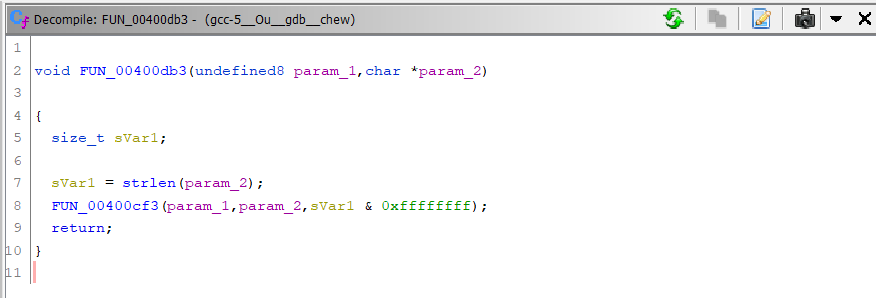
\includegraphics[width=\linewidth]{img/Nero.png}
  \caption{Short decompiled function from the GNU Debugger \cite{Nero} decompiled by Ghidra}
\end{figure}

We observe that Ghidra's decompiler manages to recover a variable name and an external call to the strlen function. In our stripped samples we do not observe this behaviour, none of the library functions is recovered and Ghidra predicts no variable names even in samples compiled using -O0.

From the intermediate-training objectives, we find that the translation task lowers performance. There could be two explanations for this: Firstly, the model is intermediately-trained on a PL-to-PL objective, while the fine-tuning objective is a PL-to-NL objective. This causes a so-called mismatch in training objectives. Recall that Transformers \ref{background} encode the input into embedding space using an encoder, the decoder will then transform this embedding into the output. In this case, this mismatch in objectives causes the decoder to be weakened in PL-to-NL tasks by the intermediate-training objective. During the pre-training phase which is applied by \citeauthor{CodeT5}, the objectives are a mix of NL-to-PL, PL-to-PL and PL-to-NL tasks. This allows a single model to be flexible and to be applied to different tasks.

The second explanation for the lower performance after TRANS intermediate-training is that the target length is also different. While the output for code summarization is at most 12 tokens long, Neural Code Translation has a target length of 512 tokens. In general, longer target sequences make it difficult for the Transformer model to properly apply the attention gradient over the entire sequence length.

The DOBF and SPAN intermediate-training objectives do yield better performance. Both of these objectives solve the objective mismatch issue and are PL-to-NL objectives. The DOBF performed slightly higher which could be explained by the shorter target length since it had no repeated identifiers.

\section{Threats to validity}

This section will cover the threats to validity. These threats are split into 3 categories. The internal threats cover threats to the validity of the study, i.e. whether the conclusions are valid within the confines of our experimental setup. The external threats cover threats to the applicability (generalisability) of our study to situations outside the confines of our experiments. Lastly, the construct validity section covers how well our work covers and measures the intended constructs.
\subsection{Internal}
    \begin{description}
        \item[Noise] The training and evaluation data contains a significant amount of noise, either in the form of badly decompiled functions or incorrect documentation. While machine learning models (and specifically NLP models) should be able to handle noisy data, this might introduce some bias into the models.
        \item[Inductive bias] The base CodeT5 model on which we applied our intermediate-training and fine-tuning strategies, will include some bias which would then be transferred to our model.
        \item[Lucky sets] The randomly selected test set might not be representative of the real distribution of the data.
        \item[Data collection] Only functions that decompile (Ghidra produces any output) and are commented are represented in the data. This is most apparent in the stripped dataset, where we are only able to recover a small fraction of the total number of functions. 
    \end{description}
\subsection{External}
    \begin{description}
        \item[Resisting analysis] This work only focuses on stripping as a means of resisting binary analysis, other techniques like control flow or data obfuscation are also used to prevent reverse engineering. 
        \item[Stripping techniques] In this work a very bipolar notion of stripping was used, the strip utility utilized removes any and all identifiers from the binary after compilation. Other techniques, which remove some identifiers before compilation, will result in different decompiled codes with some identifiers left behind by the compiler. 
    \end{description}
\subsection{Construct}
    \begin{description}
        \item[Mono-operation bias] This work only explores a single SOTA model and only focuses on NLP techniques. Other models, or other techniques, might be more successful at this task.
        \item[Mono-method bias] This work exclusively focuses on the generation of code summaries from functions to help REs understand binaries. While the code summarization task is well defined in the source-code domain, it might not be well suited for binary analysis.
    \end{description}


\section{Broader Impacts}
In this thesis we propose a novel solution to aid reverse engineers in their work. Among many use cases, this solution could help malware analysts to quickly understand novel malware and its weaknesses. The software can be analysed to find possible vulnerabilities and malicious payloads. The source code can be reconstructed for old binaries for which the source code is lost. Finally, it could help in the process of patching binary programs, known as micropatching.

The proposed solution applies a well-known and well-studied task from the software engineering research field to the binary reverse engineering domain. We have proposed a model for one of the many different applications of NLP to code. Other existing and extensively studied applications, like defect detection and code repair, could also be applied to decompiled code. 

While the proposed solution has some limitations, especially for stripped code, we hope that our work inspires other researchers to further improve our models or to propose their own solutions. For this, and in the spirit of open science, we have also published our research data. Other researchers can improve our models by designing their own pre-training objectives and applying them to an already trained model. Furthermore, researchers could also use the provided datasets to train and evaluate their own models.

\section{Ethical Considerations}
\subsection{Automation Bias}
The model that we propose can provide REs with assistance in understanding decompiled binaries. The automation bias of such a model should be carefully considered, especially since REs can over-rely on the model outputs. The output might be incorrect and could lead the RE down an incorrect path, leading to the RE requiring a longer time to understand the binary or to understand the binary incorrectly, thus missing certain important security faults or incorrectly labelling the binary as non-malicious. The output of the model should always be taken as a reference by practitioners and should always be checked for correctness.

\subsection{Offensive Language}
As we have observed in the training data, some of the comments that were mined from Github contain insulting or discriminatory statements \ref{fig:offensive}. The prevalence of offensive language in Software Engineering communities such as Github is a known issue \cite{OffensiveLanguage}. As the training data might contain such samples, this same language might be reflected in the model output. 
\label{fig:offensive}
\begin{figure}[H]
  \centering
\begin{lstlisting}
//WTF IS THIS!!!
//Are you really trying to prevent the analyzed binary 
from doing anything that would cause it to segfault irl?
//WHY?
//	- <Author removed>
\end{lstlisting}
  \caption{Example of an offensive comment from radareorg/radare2-bindings/radare2/libr/anal/esil.c, note that this comment has been removed in the most recent version}
\end{figure}


\subsection{Computational Costs}
Training these models requires a non-negligible amount of computational resources. We attempted to carefully design our experiments to limit the number of GPU hours. We also selected a pre-trained model which allows us to skip the expensive pre-training step. Compared to other state-of-the-art LLMs, CodeT5 is a relatively small model with only 220M parameters compared to CodeX which has 12B parameters \cite{CodeX}. Furthermore, we release our trained models, such that repeated training by the community can be avoided.

\subsection{Malicious Use}
As with much research in the field of binary reverse engineering, this work could be used for malicious purposes. Malicious practitioners could use this work to RE binaries and extract protected intellectual property. Furthermore, this work could be used to analyse binaries for faults and vulnerabilities, such that they can be developed into exploits for use by malicious actors. Any reverse engineer aided by the methods proposed in this work should carefully consider the legal and ethical aspects of their effort.  \footnote{Electronic Frontier Foundation: \url{https://www.eff.org/issues/coders/reverse-engineering-faq}} Furthermore, any and all vulnerabilities discovered with the help of these methods should be disclosed responsibly to the owner without needlessly putting the security of users at risk. 
\chapter{Conclusion and Future Work}
\label{conclusion}
\section{Conclusion}
% Answer the research questions according to the findings

% \section{Future Work}

% \begin{itemize}
%     \item Exploration of other compiled languages
%     \item Evaluation of different decompilers (Radare/Ida/Hopper)
%     \item Since Ghidra decompiles some functions badly and generally recovers very few additional details, exploration of the application of these methods to disassembled code instead of decompiled code
%     \item Automatic scoring methods to determine the quality of a decompiled sample
%     \item The application of semantic scoring methods to this model
%     \item Exploration of other, weaker strippers
%     \item Developing this model into a Ghidra plugin
%     \item Instead of using base Ghidra, use a different model like DIRE to add identifiers to the stripped code
% \end{itemize}
% \section{Threats to validity}
% \subsection{Internal}
% \begin{itemize}
%     \item Noise, some samples have low-quality comments (Badly written documentation, or incorrectly collected)
%     \item Inductive bias from the pre-trained base model
%     \item A lucky randomly selected test set
%     \item Bias stemming from data collection (only samples that decompile nicely and are commented are represented in the data)
% \end{itemize}
% \subsection{External} 
% \begin{itemize}
%     \item This research only covers unstripped and stripped binaries, some code, particularly malware might use methods to resist analysis
%     \item We use a very bipolar notion of stripping, some binaries might have been stripped with a significantly weaker stripper
    
% \end{itemize}
% \subsection{Construct}
% \begin{itemize}
%     \item We only cover and explore a single state-of-the-art model, other models might be more successful (mono-operation)
%     \item Documentation that can be derived from code, might not be useful at all (mono-method) (can be argued about code summarization in general)
% \end{itemize}
% \section{Ethical Considerations}
% \begin{itemize}
%     \item Automation Bias
%     \item Insulting comments in dataset can reflect in output
%     \item Non-negligible computation costs in training and deduplication, we try to limit this by providing trained models and pre-processed data
%     \item This technique, and reverse engineering techniques in general can be used for malicous purposes. 
% \end{itemize}
% \newpage
To conclude the thesis we will first answer the research questions posed in chapter \ref{methodology} based on our findings and discussion. We will then discuss possible directions for future work based on this thesis. The threats to validity will then be covered. Finally, the chapter will be closed with a short reflection on the ethical considerations and broader impact of this work.

\todo[inline]{you can avoid the bullet points here (or re-mentioning the RQs), just highlight the main findings and insights of your work in two paragraphs. also avoid two subsections with the same name}
\begin{itemize}
    \item \textbf{RQ1: How do different input types (source, unstripped decompiled, demi-stripped, stripped) affect the model's performance? (data-richness effect)}
    \begin{sloppypar}
    We found that source and unstripped decompiled code performed relatively well, while demi-stripped performed significantly worse. Stripped performed even worse and the resulting model was mostly unusable.
    \end{sloppypar}
    \item \textbf{RQ2: What is the impact of data duplication on the model's performance? (data-duplication effect)}
    \begin{sloppypar}
    We found that duplicates have a relatively large impact on the model performance, removing these duplicates puts the model performance in line with other datasets. This shows that our models are not only reproducing previously encountered summaries, but are also able to create new summaries.
    \end{sloppypar}
    \item \textbf{RQ3: To what extent does each aspect of stripped decompiled binaries impact the model's performance? (data-input study)}
    \begin{sloppypar}
    We found that the loss of identifiers causes a relatively small drop in performance. The introduction of decompilation faults in stripped code has a large impact on the model performance.
    \end{sloppypar}
    \item \textbf{RQ4: How do different intermediate-training objectives affect the model's performance? (model-objective effect)}
    \begin{sloppypar}
    We found that the performance of the model can be improved using intermediate-training objectives. Mainly, we found that a Deobfuscation intermediate-training objective improves model performance across the board. We found that the effectiveness of the intermediate-training objective is dependent on the fine-tuning objective.
    \end{sloppypar}
\end{itemize}

\section{Future Work}
This work solely focuses on the C language, these same techniques could be applied to other compliled languages. Of particular interest is the Go language, much of the novel malware is written in Go.\\
Besides the exploration of other languages, other stripping techniques could also be explored. We solely focussed on the strip tool included in Linux, but other stripping techniques, some of which are less strict than the Linux implementation, could also be explored.\\

Furthermore, we focus solely on the Ghidra decompiler, which is free to use. Other paid decompilers could also be used for the decompilation step. IDA-Pro\footnote{IDA-Pro: \url{https://hex-rays.com/ida-pro/}} features more advanced function identification methods as F.L.I.R.T.\footnote{F.L.I.R.T: \url{https://hex-rays.com/products/ida/tech/flirt/in_depth/}} and Lumina\footnote{Lumina: \url{https://hex-rays.com/products/ida/lumina/}}, which could help with function extraction in stripped binaries.\\
We found that Ghidra struggles to decompile stripped functions and generally adds very little syntax or identifiers to the function, which is why the exploration of these methods on disassembled code might see more success. Disassembled code should have fewer decompilation errors and mistakes.\\
Another solution would be to keep using these methods, but add an additional module which can determine whether a stripped sample is a well decompiled function or if a decompilation failure has occurred. The improperly decompiled functions could be skipped, and the RE would only receive the high quality output.\\
The output of Ghidra could also be enhanced using a model like DIRE \cite{Dire} or Debin \cite{Debin} to recover more identifiers, before passing the function to the summarization model. This method would however incur an additional performance penalty since it needs to decompile the binaries and recover the identifiers using one of these models.\\

The use of BLEU-4 as a scoring method also introduces some issues. The currently employed scoring methodology does not take semantics into account, meaning that the model could produce perfectly valid and usable descriptions, but since they do not match the syntax of the baseline, the score will be very low and the model will be penalized. The introduction of semantic scoring methods. Instead of using the BLEU-4 score to score the candidate against the baseline, a semantic method could also be employed. VarCLR \cite{VarCLR} can determine the semantic similarity of terms using a learned embedding. Note that there is a difference between relatedness, which some other novel solutions employ, and similarity, which VarCLR captures. \textbf{Maximum} and \textbf{Minimum} are highly related but they are not similar, one cannot be substituted with the other while preserving meaning. \textbf{Minimum} and \textbf{Minimal} are both related and similar, since they can be substituted. \\

Finally, this work could be developed into a Ghidra plugin. Using Ghidra's scripting engine, it should be relatively straightforward to extract the functions from the decompiled code and to infer the comments using one of our trained models. The script can then insert the comments to the decompiled functions in the decompiler window. The script would then be run when a binary is processed by Ghidra to aid the RE in understanding the binary.


\bibliographystyle{plainnat}
\bibliography{thesis}

\appendix
\def\chaptername{Appendix}
\chapter{\label{cha:glossary}Glossary}

In this appendix, we give an overview of frequently used terms and
abbreviations.

\begin{description}
\item[BLEU:] BiLingual Evaluation Understudy
\item[CNN: ] Convolutional Neural Network
\item[COTS: ] Commercial Off-The-Shelf
\item[DOBF:] Deobfuscation
\item[EM: ] Exact Match
\item[IR:] Intermediate Representation
\item[LLM: ] Large Language Model
\item[LSTM: ] Long Short-Term Memory
\item[MASK:] Mask Prediction
\item[ML:] Machine Learning
\item[MLM:] Masked Language Modelling
\item[NL: ] Natural Language
\item[NLP:] Natural Language Processing
\item[NMT:] Neural Machine Translation
\item[PL: ] Programming Language
\item[RE:] Reverse Engineer or Reverse Engineering
\item[RNN: ] Recurrent Neural Network
\item[seq2seq:] Sequence-to-sequence
\item[SOTA: ] State-Of-The-Art
\item[SPAN:] Span detection
\item[TL: ] Transfer Learning
\end{description}

\newpage
\chapter{\label{app:ExtremeSum} Extreme Summarisation}
In this appendix we report on the application of the extreme summarisation task on our dataset. 

\section{Methodology and Experimental Setup}
We apply the parameters and setup as provided by~\citeauthor{PolyglotCodeBERT} for the extreme summarisation task.\footnote{Model and parameters: \url{https://zenodo.org/record/5670434}} Note that the authors use their setup for the summarisation task and only change the maximum target length of the output to 10 tokens. We fine-tune a CodeBERT~\cite{CodeBERT} model for 5 epochs, we chose this limit for brevity as we found that all models converged during the third or fourth epoch as can be observed in figure~\ref{fig:ExtremeLoss}. After every epoch we evaluate the model using the validation set, and finally the model is tested using the test set.


\begin{figure}[h]
  \centering
  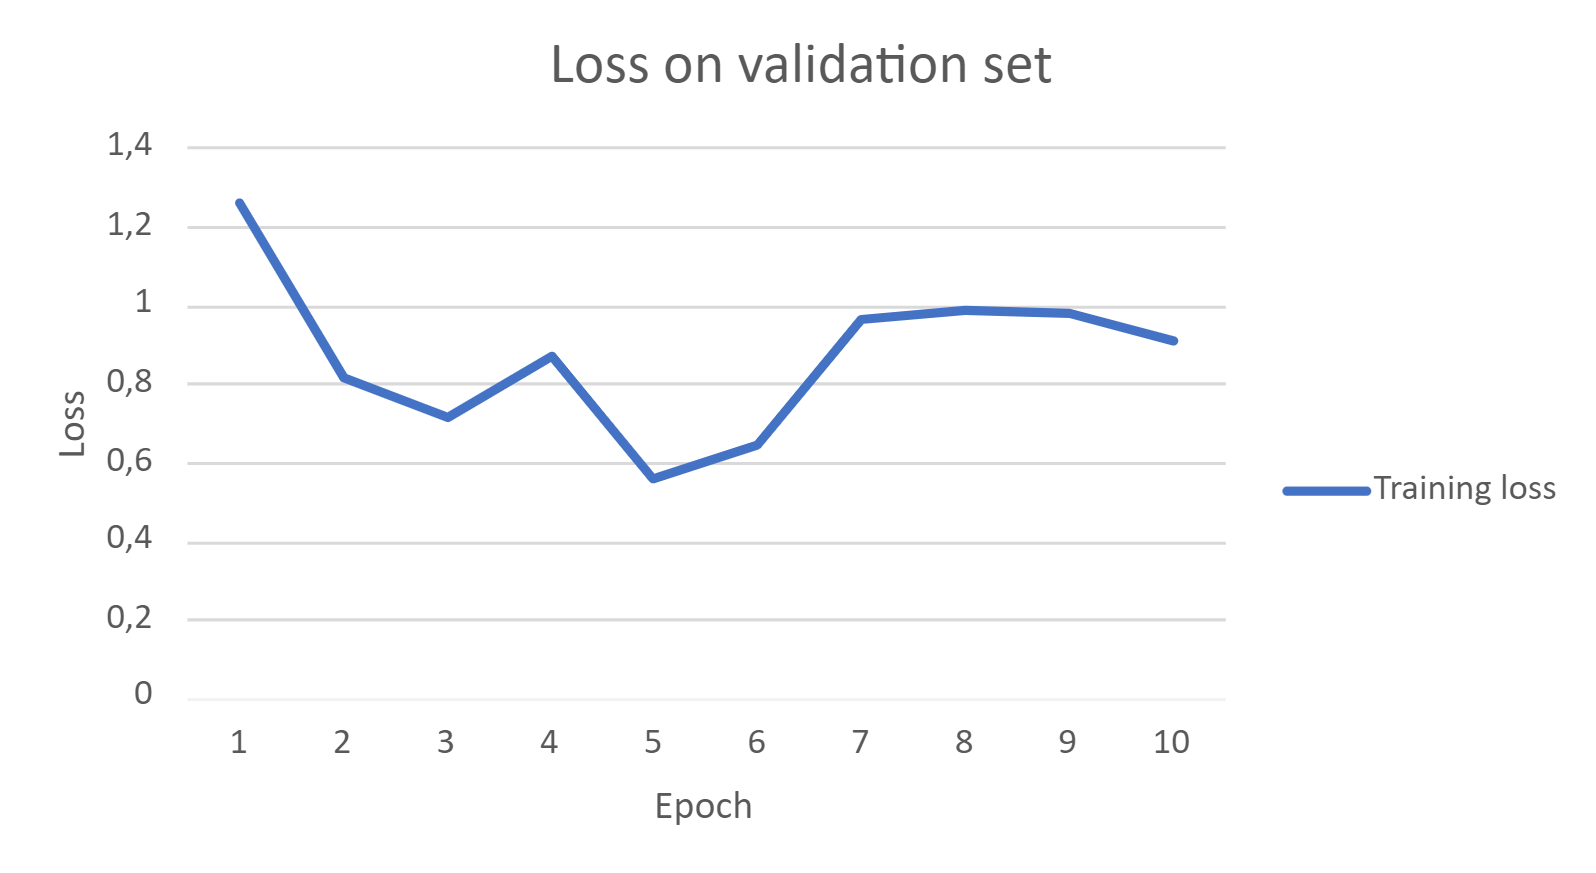
\includegraphics[width=\linewidth]{img/ExtremeLoss.png}
  \caption{Loss during CodeBERT training on stripped data}
  \label{fig:ExtremeLoss}
\end{figure}

To prepare the dataset, we use the same pipeline as shown in figure~\ref{fig:dataCollection}. Instead of extracting the comment data, the name of the functions is extracted from their aligned source code. These function names will function as reference. Since missing or unalignable documentation is no longer an issue, we are able to collect significantly more decompiled function-function name pairs. Our dataset consists of 2.1m decompiled and 630k stripped samples. Recall that unstripped decompiled functions still retain the function name after decompilation, so we selectively strip away the function name from the function definition and any recursive calls in the function bodies. 

The dataset is split into a train, test and validation set. Similarly to the regular summarisation task we split them in a cross-project manner, with the sets constituting 80\%, 10\% and 10\% of the complete dataset respectively. We followed the recommendations by~\citeauthor{recommend_summarization} on the dataset construction. 

Since the output of the model is so short and generally contains up to 3 tokens~\cite{ExtremeSummarization}, BLEU would be unfit as a metric. Similarly to \citeauthor{ExtremeSummarization} and \citeauthor{PolyglotCodeBERT}, we chose to use the F1-score.
\[\mathit{F1} = \frac{2*\mathit{Precision}*\mathit{Recall}}{\mathit{Precision}+\mathit{Recall}} * 100\] 
Every function name is broken up into subtokens, the name "popStack'' would therefore be tokenised into "pop" and "stack". The precision and recall are then calculated by comparing the tokens in the reference and the model prediction. Note that this does not take the order of the tokens into account.

\citeauthor{PolyglotCodeBERT} report F1 scores ranging from 24 to 54 and F1 scores ranging from 0.41 and 0.54 with regular CodeBERT and PolyglotCodeBERT respectively. Note that these models were trained and evaluated on the CodeXGLUE~\cite{CodeXGlue} dataset which is deduplicated, while our own dataset is not. %Find limit for unusable samples

\section{Results}
We find that the results resembled the results from the regular code summarisation task. The CodeBERT model achieved an F1 score of 20.6 and 5.45 on the stripped and unstripped code respectively. Manual assessment of the produced samples shows that the model for unstripped code could produce some usable samples, but the stripped model was unable to produce almost anything of value, as can be observed in table~\ref{fig:extremesumex}.

\begin{table}[tbh]
\begin{tabular}{l|ll}
\multicolumn{1}{c|}{Reference} & \multicolumn{1}{c}{Decom} & \multicolumn{1}{c}{Stripped} \\ \hline
main                           & main                      & main                         \\
sha 256 transform              & md 5  process  block      & sha 1  process  block        \\
get ins len                    & op nd  num  reg s         & op nd  get  size             \\
r id storage foreach           & queue  fore ach           & hash  find                   \\
map init                       & pro g  init               & c se g  open                
\end{tabular}
\caption{Sample of CodeBERT extreme summarisation model output}
\label{fig:extremesumex}
\end{table}

% \chapter{Requirements and Guidelines}

This chapter details some requirements and guidelines for MSc theses
submitted to the Software Engineering Research Group.

\section{Requirements}

\subsection{Layout}

\begin{itemize}
\item Your thesis should contain the formal title pages included in
  this document (the page with the TU Delft logo and the one that
  contains the abstract, student id and thesis committee). Usually
  there is also a cover page containing the thesis title and the
  author (this document has one) but this can be omitted if desired.
 
\item Base font should be an 11 point serif font (such as Times, New
  Century Schoolbook or Computer Modern). Do not use sans-serif fonts
  such as Arial or Helvetica. \textsl{Sans-serif type is intrinsically
  less legible than seriffed type} \cite{Whe95}.

\item The final thesis and drafts submitted for reviewing should be
printed double-sided on A4 paper.
\end{itemize}

\subsection{Content}

\begin{itemize}
\item The thesis should contain the following chapters:
\begin{itemize}
\item Introduction.

  Describes project context, goals and your research question(s). In
  addition it contains an overview of how (the remainder of) your
  thesis is structured.

\item One or (usually) more ``main'' chapters.

  Present your work, the experiments conducted, tool(s) developed,
  case study performed, etc.

\item Overview of Related Work

  Discusses scientific literature related to your work and describes
  how those approaches differ from what you did.

\item Discussion/Evaluation/Reflection

  What went well, what went less well, what can be improved?

\item Conclusions, Contributions, and (Recommendations for) Future Work

\item Bibliography

\end{itemize}
\end{itemize}


\subsection{Bibliography}

\begin{itemize}
\item Make sure you've included all required data such as journal,
  conference, publisher, editor and page-numbers. When you're using
  \textsc{Bib}\TeX{}, this means that it won't complain when running
  \texttt{bibtex your-main-tex-file}.
 
\item Make sure you use proper bibliographic references. This
  especially means that you should avoid references that \textbf{only}
  point at a website and not at a printed publication.

  For example, it's OK to add a URL with the entry for an article
  describing a tool to point at its homepage, but it's not OK to just
  use the URL and not mention the article.
\end{itemize}


\section{Guidelines}

\begin{itemize}

\item The main chapters of a typical thesis contain approximately 50
  pages.

\item A typical thesis contains approximately 50 bibliographic
  references.

\item Make sure your thesis structure is balanced (check this in the
  table of contents). 

  Typically the main chapters should be of equal length. If they aren't,
  you might want to revise your structure by merging or splitting some
  chapters/sections.

  In addition, the (sub)section hierarchies with the chapters should
  typically be balanced and of similar depth. If one or more are much
  deeper nested than others in the same chapter this generally signals
  structuring problems.

\item Whenever you submit a draft of your thesis to your supervisor
  for reviewing, make sure that you have checked the spelling and
  grammar.  Moreover, \emph{read it yourself at least once from start
  to end, before submitting to your supervisor}.

  \textbf{Your supervisor is not a spelling/grammar checker!}

\item Whenever you submit a second draft, include a short text which
  describes the changes w.r.t. the previous version. 

\end{itemize}






\end{document}
